\documentclass[
  parskip=half,           % halbzeiliger Zeileneinzug nach Absatz
  bibliography=totoc,     % Literatur im Inhaltsverzeichnis
  captions=tableheading,  % Tabellenüberschriften
  titlepage=firstiscover, % Titelseite ist Deckblatt
]{scrartcl}

\usepackage{geometry}
\geometry{a4paper,left=25mm,right=25mm, top=3cm, bottom=3cm}

% Paket float verbessern
\usepackage{scrhack}

% Warnung, falls nochmal kompiliert werden muss
\usepackage[aux]{rerunfilecheck}

% deutsche Spracheinstellungen
\usepackage{polyglossia}
\setmainlanguage{german}

% unverzichtbare Mathe-Befehle
\usepackage{amsmath}
% viele Mathe-Symbole
\usepackage{amssymb}
% Erweiterungen für amsmath
\usepackage{mathtools}

% Fonteinstellungen
\usepackage{fontspec}
% Latin Modern Fonts werden automatisch geladen

\usepackage[
  math-style=ISO,    % ┐
  bold-style=ISO,    % │
  sans-style=italic, % │ ISO-Standard folgen
  nabla=upright,     % │
  partial=upright,   % ┘
  warnings-off={           % ┐
    mathtools-colon,       % │ unnötige Warnungen ausschalten
    mathtools-overbracket, % │
  },                       % ┘
]{unicode-math}

% traditionelle Fonts für Mathematik
\setmathfont{Latin Modern Math}
\setmathfont{XITS Math}[range={scr, bfscr}]
\setmathfont{XITS Math}[range={cal, bfcal}, StylisticSet=1]

% Zahlen und Einheiten
\usepackage[
  locale=DE,                 % deutsche Einstellungen
  separate-uncertainty=true, % immer Fehler mit \pm
  per-mode=reciprocal,       % ^-1 für inverse Einheiten
  % alternativ:
  % per-mode=reciprocal, % m s^{-1}
  % decimal-marker=., % . statt , f�r Dezimalzahlen
]{siunitx}

% chemische Formeln
\usepackage[
  version=4,
  math-greek=default, % ┐ mit unicode-math zusammenarbeiten
  text-greek=default, % ┘
]{mhchem}

% tikzpicture ("Zeichenprogramm")
\usepackage{tikz}
\usetikzlibrary{circuits.ee.IEC}
\usetikzlibrary{positioning}
\tikzset{
  Pfeil/.style={thick,shorten >=#1,shorten <=#1,->,>=latex}, % für Peile
  UPfeil/.style={blue,Pfeil=#1,font={\sffamily\itshape}},% für Spannungspfeile
  IPfeil/.style={red,Pfeil=#1,font={\ttfamily\itshape}} % für Strompfeile
}
%Volt- und Amperemeter festlegen:
\tikzset{circuit declare symbol = Us}
\tikzset{set Us graphic ={draw,generic circle IEC, minimum size=5mm,info=center:$U_s$}}

\tikzset{circuit declare symbol = voltmeter}
\tikzset{set voltmeter graphic ={draw,generic circle IEC, minimum size=5mm,info=center:V}}

% richtige Anführungszeichen
\usepackage[autostyle]{csquotes}

% schöne Brüche im Text
\usepackage{xfrac}

\usepackage{blindtext}    % \blindtext zum Testen von Texten.

% Standardplatzierung für Floats einstellen
\usepackage{float}
\floatplacement{figure}{htbp}
\floatplacement{table}{htbp}

% Floats innerhalb einer Section halten
\usepackage[
  section, % Floats innerhalb der Section halten
  below,   % unterhalb der Section aber auf der selben Seite ist ok
]{placeins}

% Seite drehen für breite Tabellen
\usepackage{pdflscape}

% mehrere Seiten einer einzelnen pdf, zB
% \includepdf[pages={1-2}]{Bilder/Messdaten.pdf}
\usepackage{pdfpages}

% Captions schöner machen.
\usepackage[
  labelfont=bf,        % Tabelle x: Abbildung y: ist jetzt fett
  font=small,          % Schrift etwas kleiner als Dokument
  width=0.9\textwidth, % maximale Breite einer Caption schmaler
  %indention=1cm        % Einrückung nach der ersten Zeile
]{caption}
% subfigure, subtable, subref
\usepackage{subcaption}

% mit Buchstabend gelistete items: \begin{enumerate}[label={\alph*)}]
\usepackage{enumitem}

% Grafiken können eingebunden werden
\usepackage{graphicx}
% größere Variation von Dateinamen möglich (Probleme mit Leerzeichen behoben)
\usepackage{grffile}

% schöne Tabellen
\usepackage{booktabs}
\sisetup{table-format=1.2}
%\begin{tabular}{S[table-format=3.0] S S S S[table-format=3.2]}
%table-format : 3 stellen vor, 0 stellen nach dem Komma
% S steht f�r siunix, dh. wir verwenden solche Zahlen
% \multicolumn{2}{c}{Spalte 1}
% wie in excel Spalten zusammenf�gen
% Einheiten: {$\lambda \:/\: \si{\nano\meter}$}

% Uncertainties:
%\begin{tabular}{
% S[table-format=3.1]
% @{${}\pm{}$}
% S[table-format=2.1]
% }
% \toprule
% \multicolumn{2}{c}{$x \:/\: \si{\ohm}$} \\
% \midrule
% 632.4 & 5.7 \\

% Verbesserungen am Schriftbild
\usepackage{microtype}

% Literaturverzeichnis
\usepackage[
  backend=biber,
]{biblatex}
% Quellendatenbank
\addbibresource{Quellen.bib}
\addbibresource{programme.bib}

% Hyperlinks im Dokument
\usepackage[
  unicode,        % Unicode in PDF-Attributen erlauben
  pdfusetitle,    % Titel, Autoren und Datum als PDF-Attribute
  pdfcreator={},  % ┐ PDF-Attribute säubern
  pdfproducer={}, % ┘
  linkcolor=blue, % einfache interne Verkn?pfungen
  citecolor=blue, % Verweise auf Literaturverzeichniseintr?ge im Text
]{hyperref}
% erweiterte Bookmarks im PDF
\usepackage{bookmark}

% Trennung von Wörtern mit Strichen
\usepackage[shortcuts]{extdash}

\author{
  Marius Hötting%
  \texorpdfstring{
    \\
    \href{mailto:Marius.Hoetting@udo.edu}{Marius.Hoetting@udo.edu}
  }{}%
  \texorpdfstring{\and}{, }
  Matthias Jaeger%
  \texorpdfstring{
    \\
    \href{mailto:Matthias.Jaeger@udo.edu}{Matthias.Jaeger@udo.edu}
  }{}%
}
\publishers{TU Dortmund – Fakultät Physik}


% TYPOGRAPHIE:

% Nutze z.\,B. um Zeilenumbruch zu verhindern.
% Gedankenstriche mit --  (statt -)
% \\[2\baselineskip] erstellt einen vspace mit 2 Baselines, also 2 Zeilen


% \renewcommand{\baselinestretch}{1.3}										%Zeilenabstand


% zu breite Tabellen/Figures:
%\OverfullCenter{
%  \begin{figure}
%   ...
%  \end{figure}
%}
\NewDocumentCommand \OverfullCenter {+m} {
  \noindent\makebox[\linewidth]{#1} }



% Klammern werden nach außen hin leicht größer gesetzt.
\setlength{\delimitershortfall}{-1sp}


% Zusammenfassung neue Dinge: \Re(x)  \Im(x)  \v{x} \dif{x} \Dif{x}
% des weiteren werden in Mathebefehle.tex weitere Sachen definiert
% This work is licensed under the Creative Commons
% Attribution-NonCommercial 3.0 Unported License. To view a copy of this
% license, visit http://creativecommons.org/licenses/by-nc/3.0/.

% equation environments
\newenvironment{eqn}{\begin{eqns}[c]}{\end{eqns}\ignorespacesafterend}
\newenvironment{eqn*}{\begin{eqns*}[c]}{\end{eqns*}\ignorespacesafterend}
\newenvironment{eqns}[1][rCl]{\begin{IEEEeqnarray*}{#1}}{\end{IEEEeqnarray*}\ignorespacesafterend}
\newenvironment{eqns*}[1][rCl]{\begin{IEEEeqnarray}{#1}}{\end{IEEEeqnarray}\ignorespacesafterend}

% Differentialrechnung
\renewcommand{\d}{\ensuremath{\mathrm{d}}}

% Totale Ableitungen
\newcommand{\td}[2]{\ensuremath{\frac{\d{#1}}{\d{#2}}}}
\newcommand{\tdd}[2]{\ensuremath{\frac{\d^2{#1}}{\d{#2}^2}}}

% Partielle Ableitungen
\newcommand{\pd}[2]{\ensuremath{\frac{\partial{#1}}{\partial{#2}}}}
\newcommand{\pdd}[2]{\ensuremath{\frac{\partial^2{#1}}{\partial{#2}^2}}}

% Der Körper der reellen Zahlen
\newcommand{\R}{\ensuremath{\mathbb{R}}}

% Der Körper der natürlichen Zahlen
\newcommand{\N}{\ensuremath{\mathbb{N}}}

% Der Körper der komplexen Zahlen
\renewcommand{\C}{\ensuremath{\mathbb{C}}}

% Imaginäre Einheit
\newcommand{\iu}{{\mathrm{i}\mkern1mu}}

%Real- und Imaginärteil vernünftig mit \Re und \Im
\AtBeginDocument{ % wird bei \begin{document} ausgeführt
\let\symIm=\Im % werden sonst wieder von unicode-math überschrieben
\RenewDocumentCommand \Re {}
{
  \operatorname{Re}
}
\let\symIm=\Im
\RenewDocumentCommand \Im {}
{
  \operatorname{Im}
}
}


% mit \abs{x} und \norm{x} arbeiten
\DeclarePairedDelimiter{\abs}{\lvert}{\rvert}
\DeclarePairedDelimiter{\norm}{\lvert}{\rvert}


%\dif[x]{t}  : totale Ableitung von x nach t
\NewDocumentCommand \dif {O{leck mich} m}
{
  \frac{\mathinner{\symup{d} #1}} {\mathinner{\symup{d} #2}}
}

%\Dif{x}  : totale Ableitung von x
\NewDocumentCommand \Dif {m}
{
  \mathinner{\symup{D} #1}
}

% Mathemodus schönere Buchstaben mit \v{t}
\let\vaccent=\v % alten Befehl kopieren
\RenewDocumentCommand \v {} % Befehl überschreiben
{
  \TextOrMath{
    \vaccent % Textmodus
    }{
      \symbf
      }
}



\subject{V60}
\title{Diodenlaser}
\date{
  Durchführung: 01.02.2019
  \hspace{3em}
  Abgabe: 11.02.2019
}

\begin{document}

\maketitle
\thispagestyle{empty}
\tableofcontents
\newpage

\section{Theorie}
\label{sec:Theorie}

Damit eine elektromagnetische Welle zur Informationsübertragung verwendet werden kann, wird eine hochfrequenten Trägerspannung mit einer niederfrequenten Modulationsspannung kombiniert. Diese Kombination kann zum einen durch die Modulierung der Frequenz oder zum anderen durch die Modulierung der Amplitude beider Spannung erzeugt werden. Unter Verwendung mehrerer Trägerspannungen ist es möglich verschiedene Informationen gleichzeitig zu übertragen, wie z.B. bei den Funkkanälen des Radios. Zur Extraktion der Information der Welle am Empfangsort wird die Demodulation angewandt. Die Grundlagen der zuvor angesprochenen Frequenz- und Amplitudenmodulation bzw. Demodulation werden in Kapitel \ref{sec:Amplitudenmodulation} und \ref{sec:Frequenzmodulation} erläutert.

\subsection{Amplitudenmodulation}
\label{sec:Amplitudenmodulation}

Bei dieser Methode der Modulation führt die Amplitude einer hochfrequenten Trägerspannung Schwingungen im Rhythmus der niederfrequenten Modulationsspannung, die die Informationen enthält, aus. Beschrieben werden die beiden verwendeten Spannungen durch die Gleichungen 
\begin{align}
	U_T(t)=\hat{U}_T\cos{(\omega_Tt)} \;\; \text{und} \;\; U_M(t)=\hat{U}_M\cos{(\omega_Mt)}\; ,
\end{align}
dabei bezeichnet $U_T$ die Trägerspannung, $U_M$ die Modulationsspannung, $\omega_T$ die Trägerfrequenz und $\omega_M$ die Modulationsfrequenz. Durch die Kombination der Spannungen ergibt sich
\begin{align}
	U(t)=\hat{U}_T(1+m\cos{(\omega_M)})\cos{(\omega_Tt)}\;.
	\label{eq:1}
\end{align}

Der mit $m$ bezeichnete Modulationsgrad ist über die Amplitude der Modulationsspannung wie folgt definiert:
\begin{align}
	m=\gamma\hat{U}_M \;\; \text{mit} \;\; m= [0,1]
\end{align}
Wie in Abbildung \ref{fig_T1} zu sehen, ergibt sich unter Betrachtung der Extremwerte 
\begin{align}
	\hat{U}_T(1-m) \;\; \text{und} \;\; \hat{U}_T(1+m)\;,
\end{align}
die abgebildete amplitudenmodulierte Spannung des Signals. 

\begin{figure}
    \centering
    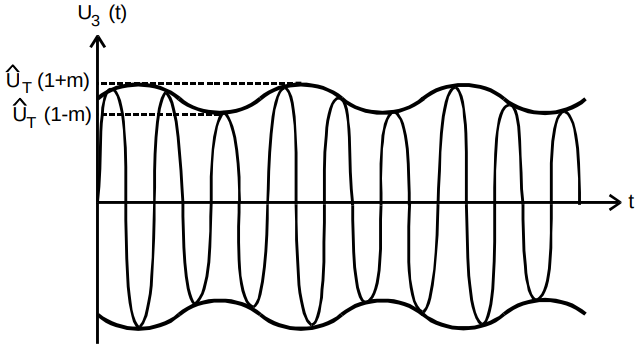
\includegraphics[width=0.55\textwidth]{ressources/T1.png}
    \caption{Darstellung einer amplitudenmodulierten Spannung in Abhängigkeit der Zeit $t$\cite{skript}.}
    \label{fig_T1}
\end{figure}

Um das Frequenzspektrum dieser Schwingung zu ermitteln, wird Gleichung \eqref{eq:1} mittels trigonometrischen Beziehungen zu
\begin{align}
	U(t)=\hat{U}_T\left(\cos{(\omega_Tt)+\frac{1}{2}m\cos{(\omega_T+\omega_M)t}}+\frac{1}{2}m\cos{(\omega_T-\omega_M)t})\right)
\end{align}
vereinfacht. Somit besteht das Frequenzspektrum aus den drei Frequenzen
\begin{align}
	\omega_T-\omega_M,\quad\omega,\quad\omega_T+\omega_M\;.
\end{align}
In Abbildung \ref{fig_T2} sind die zuvor beschriebenen Kreisfrequenzen gegen die Spannung aufgetragen.

\begin{figure}
    \centering
    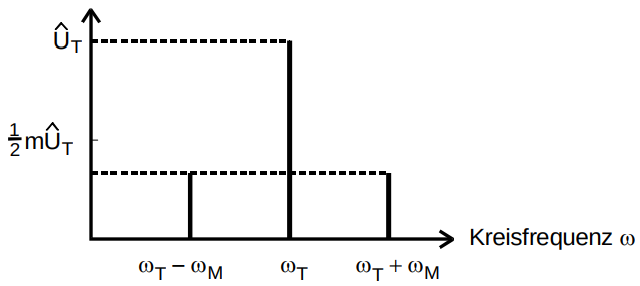
\includegraphics[width=0.55\textwidth]{ressources/T2.png}
    \caption{Darstellung eines Frequenzspektrums einer amplitudenmodulierten Spannung\cite{skript}.}
    \label{fig_T2}
\end{figure}

Bei der Betrachtung des Spektrums ist zu beachten, dass, wie auch in Abbildung \ref{fig_T2} zu sehen, die äußeren beiden Frequenzen, die sogenannten Seitenbänder, identische Informationen enthalten. Im Gegensatz dazu enthält die Frequenz $\omega_T$, die sogenannte Trägerabstrahlung, durch die fehlende Abhängigkeit von $\omega_M$ keine Information. Besteht der Umstand, dass $\omega_M$ nicht nur aus einer sondern aus einer Kombination mehrerer Frequenzen besteht, verbreitern sich die Seitenbänder in Abbildung \ref{fig_T2}. Nachteile der Amplitudenmodulation sind unter anderem die geringe Störsicherheit und die geringe Verzerrungsfreiheit. Beispielsweise kann es in engen Schaltkreise mit mangelnder Abschirmung zur Induktion einer Fremdspannung kommen, wodurch die Amplitude der Modulation beeinflusst wird. Unbeeinflusst bleibt die Frequenz, weshalb im Folgenden die Frequenzmodulation beschrieben wird.

\subsection{Frequenzmodulation}
\label{sec:Frequenzmodulation}
Bei der Frequenzmodulation entsteht eine Änderung der Trägerfrequenz verursacht durch ein Modulationssignal. Dabei ist zu betonen, dass nur die Frequenz eine Variation erfährt und die Amplitude konstant bleibt. Die modulierte Spannung kann wie folgt dargestellt werden:
\begin{align}
	U(t)=\hat{U}\sin{\left(\omega_Tt+m\frac{\omega_T}{\omega_M}\cos{(\omega_Mt)}\right)}
	\label{eq:2}
\end{align}
Die Momentanfrequenz wird dabei beschrieben durch
\begin{align}
	f(t)=\frac{\omega_T}{2\pi}(1-m\sin{(\omega_Mt)})\;.
\end{align}
Mit dem Frequenzhub
\begin{align}
	\Delta f=\frac{m\omega_T}{2\pi}
\end{align}
wird die Variationsbreite, also ein Maß für die Variation der Frequenz definiert. In Abbildung \ref{fig_T3} ist beispielhaft eine Frequenzmodulierte Schwingung skizziert.

\begin{figure}
    \centering
    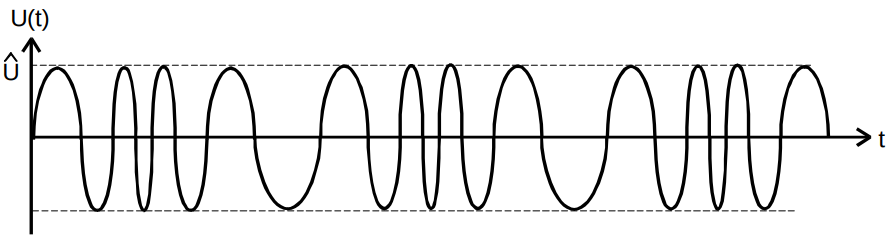
\includegraphics[width=0.85\textwidth]{ressources/T3.png}
    \caption{Darstellung einer frequenzmodulierten Spannung in Abhängigkeit der Zeit $t$\cite{skript}.}
    \label{fig_T3}
\end{figure}

Anhand einer sogenannten Schmalband-Frequenzmodulation, bei der gilt 
\begin{align}
	m\frac{\omega_T}{\omega_M}<<1,
\end{align}
soll im folgende grundlegende Eigenschaften der Frequenzmodulation verdeutlicht werden. Mittels trigonometrischer Funktionen wird Gleichung \eqref{eq:2} umgeformt zu
\begin{align}
	U(t)=\hat{U}\left(\sin{(\omega_Tt)}\cos{\left(m\frac{\omega_T}{\omega_M}\cos{(\omega_Mt)}\right)} + \cos{(\omega_Tt)}\sin{\left(m\frac{\omega_T}{\omega_M}\cos{(\omega_Mt)}\right)}\right) \:.
\end{align}
Mit einer Reihenentwicklung der Sinus- und Cosinustherme, bei der nur Therme erster Ordnung betrachtet werden, entsteht die folgende Gleichung
\begin{align}
	U(t)=\hat{U}\left(\sin{(\omega_Tt)+\frac{1}{2}m\frac{\omega_T}{\omega_M}\cos{(\omega_T+\omega_M)t}}+\frac{1}{2}m\frac{\omega_T}{\omega_M}\cos{(\omega_T-\omega_M)t})\right)\;,
\end{align}
die sehr große Ähnlichkeit zur amplitudenmodulierten Spannung aufweist, da auch hier das Frequenzspektrum aus den drei Frequenzen
\begin{align}
	\omega_T-\omega_M,\quad\omega,\quad\omega_T+\omega_M\;
\end{align}
besteht. Der wesentliche Unterschied besteht jedoch in der Trägerschwingung, da diese durch den Sinus um $90^{\circ}\text{C}$ Phasenverschoben wird.
Unter Berücksichtigung höherer Therme in der Reihenentwicklung ergibt sich 
\begin{align}
	U(t)=\hat{U}\sum_{n=-\infty}^{\infty} J_n\left(m\frac{\omega_T}{\omega_M}\right)\sin{(\omega_T+n\omega_M)}t\;. 
	\label{eq:3}
\end{align}
Der Ausdruck $J_n(x)$ steht dabei für die Besselfunktion n-ter Ordnung. Bei der Betrachtung von Gleichung \eqref{eq:3} fällt auf, dass der Iterator der Summe in der Sinusfunktion ein beliebig großes Frequenzspektrum ermöglicht. Da jedoch die Besselfunktion für steigende $n$ gegen Null strebt müssen nur Frequenzen nahe der Trägerfrequenz $\omega_T$ berücksichtigt werden.


% 2x2 Plot
% \begin{figure*}
%     \centering
%     \begin{subfigure}[b]{0.475\textwidth}
%         \centering
%         \includegraphics[width=\textwidth]{Abbildungen/Schaltung1.pdf}
%         \caption[]%
%         {{\small Schaltung 1.}}
%         \label{fig:Schaltung1}
%     \end{subfigure}
%     \hfill
%     \begin{subfigure}[b]{0.475\textwidth}
%         \centering
%         \includegraphics[width=\textwidth]{Abbildungen/Schaltung2.pdf}
%         \caption[]%
%         {{\small Schaltung 2.}}
%         \label{fig:Schaltung2}
%     \end{subfigure}
%     \vskip\baselineskip
%     \begin{subfigure}[b]{0.475\textwidth}
%         \centering
%         \includegraphics[width=\textwidth]{Abbildungen/Schaltung4.pdf}    % Zahlen vertauscht ... -.-
%         \caption[]%
%         {{\small Schaltung 3.}}
%         \label{fig:Schaltung3}
%     \end{subfigure}
%     \quad
%     \begin{subfigure}[b]{0.475\textwidth}
%         \centering
%         \includegraphics[width=\textwidth]{Abbildungen/Schaltung3.pdf}
%         \caption[]%
%         {{\small Schaltung 4.}}
%         \label{fig:Schaltung4}
%     \end{subfigure}
%     \caption[]
%     {Ersatzschaltbilder der verschiedenen Teilaufgaben.}
%     \label{fig:Schaltungen}
% \end{figure*}

\clearpage
\newpage


\printbibliography

\clearpage
\newpage
% % % \begin{appendix}
% % % \section{Messdaten}
% % % \centering
% % % \begin{figure}
% % % \includepdf[width=0.9\textwidth, pages={1}]{Bilder/Messdaten.pdf}
% % % \end{figure}
% % % \newpage
% % % \begin{figure}
% % % \includepdf[width=0.9\textwidth, pages={2}]{Bilder/Messdaten.pdf}
% % % \end{figure}
% % %
% % % \end{appendix},


% % % % Standard Plot
% \begin{figure}
%   \centering
%   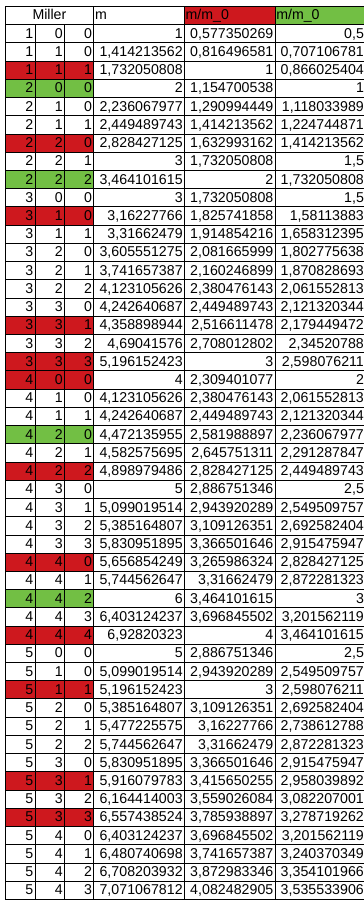
\includegraphics{ressources/Steinsalz.png}
%   \caption{Millerindizes und das theoretische Verhältnis nach \ref{eq:dm} für die Steinsalz/Fluorit-Struktur (a). Die grün hinterlegten Felder stellen schwache und die rot hinterlegten Felder starke Reflexe dar.}
%   \label{fig:Anhang1}
% \end{figure}

% \begin{figure}
%   \centering
%   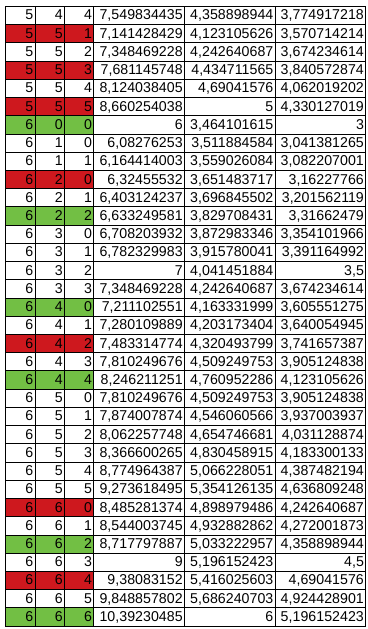
\includegraphics{ressources/Steinsalz2.png}
%   \caption{Millerindizes für die Steinsalz/Fluorit-Struktur (b).}
%   \label{fig:Anhang2}
% \end{figure}

% \begin{figure}
%   \centering
%   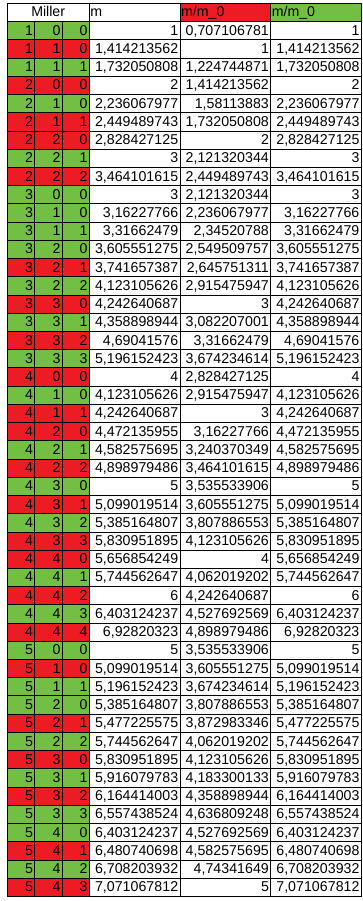
\includegraphics{ressources/Caesium.png}
%   \caption{Millerindizes und das theoretische Verhältnis nach \ref{eq:dm} für die Caesium-Struktur (a). Die grün hinterlegten Felder stellen schwache und die rot hinterlegten Felder starke Reflexe dar.}
%   \label{fig:Anhang3}
% \end{figure}

% \begin{figure}
%   \centering
%   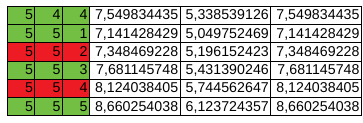
\includegraphics{ressources/Caesium2.png}
%   \caption{Millerindizes für die Caesium-Struktur (b).}
%   \label{fig:Anhang4}
% \end{figure}

% \begin{figure}
%   \centering
%   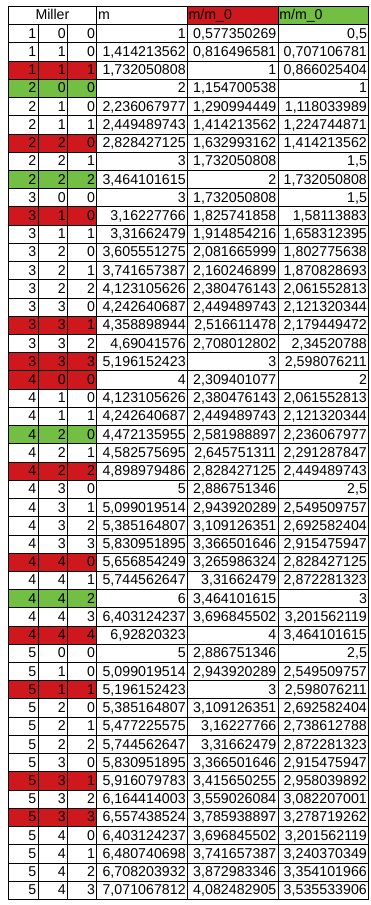
\includegraphics{ressources/Zinkblende.png}
%   \caption{Millerindizes und das theoretische Verhältnis nach \ref{eq:dm} für die Zinkblende-Struktur (a). Die grün hinterlegten Felder stellen schwache und die rot hinterlegten Felder starke Reflexe dar.}
%   \label{fig:Anhang5}
% \end{figure}

% \begin{figure}
%   \centering
%   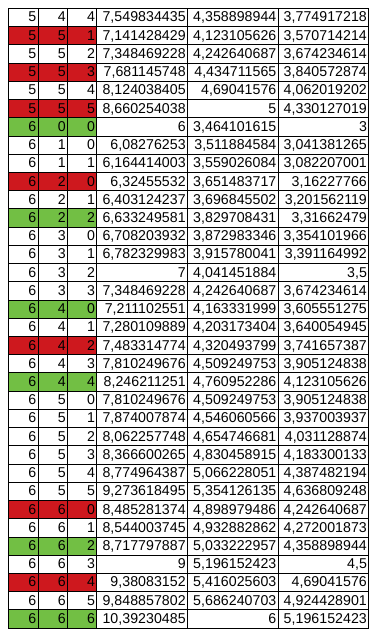
\includegraphics{ressources/Zinkblende2.png}
%   \caption{Millerindizes für die Zinblenden-Struktur (b).}
%   \label{fig:Anhang6}
% \end{figure}

\end{document}


% % Examples
% \begin{equation}
%   U(t) = a \sin(b t + c) + d
% \end{equation}
%
% \begin{align}
%   a &= \input{a.tex} \\
%   b &= \input{b.tex} \\
%   c &= \input{c.tex} \\
%   d &= \input{d.tex} .
% \end{align}
% Die Messdaten und das Ergebnis des Fits sind in Abbildung~\ref{fig:plot} geplottet.
%
% %Tabelle mit Messdaten
% \begin{table}
%   \centering
%   \caption{Messdaten.}
%   \label{tab:data}
%   \sisetup{parse-numbers=false}
%   \begin{tabular}{
%     S[table-format=1.3]
%     S[table-format=-1.2]
%     @{${}\pm{}$}
%     S[table-format=1.2]
%     @{\hspace*{3em}\hspace*{\tabcolsep}}
%     S[table-format=1.3]
%     S[table-format=-1.2]
%     @{${}\pm{}$}
%     S[table-format=1.2]
%   }
%     \toprule
%     {$t \:/\: \si{\milli\second}$} & \multicolumn{2}{c}{$U \:/\: \si{\kilo\volt}$\hspace*{3em}} &
%     {$t \:/\: \si{\milli\second}$} & \multicolumn{2}{c}{$U \:/\: \si{\kilo\volt}$} \\
%     \midrule
%     \input{table.tex}
%     \bottomrule
%   \end{tabular}
% \end{table}
%
% % Standard Plot
% \begin{figure}
%   \centering
%   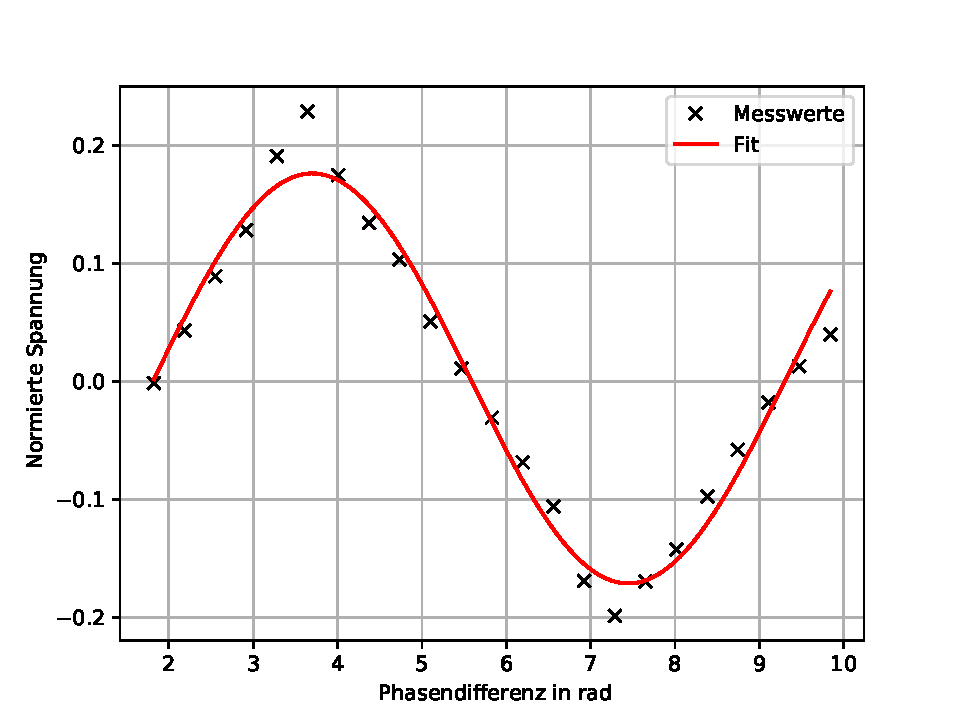
\includegraphics{plot.pdf}
%   \caption{Messdaten und Fitergebnis.}
%   \label{fig:plot}
% \end{figure}
